\documentclass[a4paper,11pt]{scrartcl}
%\documentclass[a4paper,11pt]{article}
%\documentclass{article}
%\usepackage{ams}


\usepackage{fancyhdr, blindtext}
\usepackage{hyperref}
\usepackage{url}
\usepackage{graphicx}
%\usepackage{booktabs}
\usepackage{tabularx}
\usepackage{longtable}
\usepackage[utf8]{inputenc}
\usepackage{latexsym}
\usepackage{eurosym}
\usepackage{xspace} 
\usepackage{algorithmic}
\usepackage{algorithm}
\usepackage{listings}
\usepackage{verbatim}
\usepackage{tikz}
\usetikzlibrary{calc,shapes,arrows,fit,calc,positioning,automata}

\usepackage{colortbl}
\usepackage{ulem}
\usepackage{verbatim}
\usepackage{multirow}
\usepackage{colortbl}
\usetikzlibrary{arrows,snakes}
\usepackage[margin=2.0cm,tmargin=2.5cm,bmargin=3.5cm]{geometry}

\newcommand{\changefont}[3]{
\fontfamily{#1} \fontseries{#2} \fontshape{#3} \selectfont}
 \renewcommand{\familydefault}{\sfdefault}

\newcommand{\authEnc}{Authenticated Encryption\xspace}
\newcommand{\bacpa}{BACPA\xspace}

\newcommand{\stateUninit}{\textsc{uninitialized}\xspace}
\newcommand{\stateInit}{\textsc{initialized}\xspace}
\newcommand{\stateCreated}{\textsc{constructed}\xspace}
\newcommand{\stateDestroyed}{\textsc{destroyed}\xspace}
%\input{../../phd/thesis/newcmds.tex}
\newcommand{\paper}[1]{#1}

\definecolor{csblue}{rgb}{0.32,0.47,0.85}
\definecolor{csbluelightformer}{rgb}{0.37,0.47,0.74}
\definecolor{csbluelight}{rgb}{0.41,0.52,0.81}
\definecolor{csorange}{rgb}{0.95,0.56,0.25}
\fancyhead{}
%\fancyfoot{}

\fancyheadoffset[L]{0.9cm}
\fancyheadoffset[R]{0.4cm}
\renewcommand{\headrule}{\hbox to\headwidth{%
  \color{csbluelight}\leaders\hrule height \headrulewidth\hfill}}

\renewcommand{\headrulewidth}{1.2pt}
\fancyhead[R]{\hspace{-1.9cm}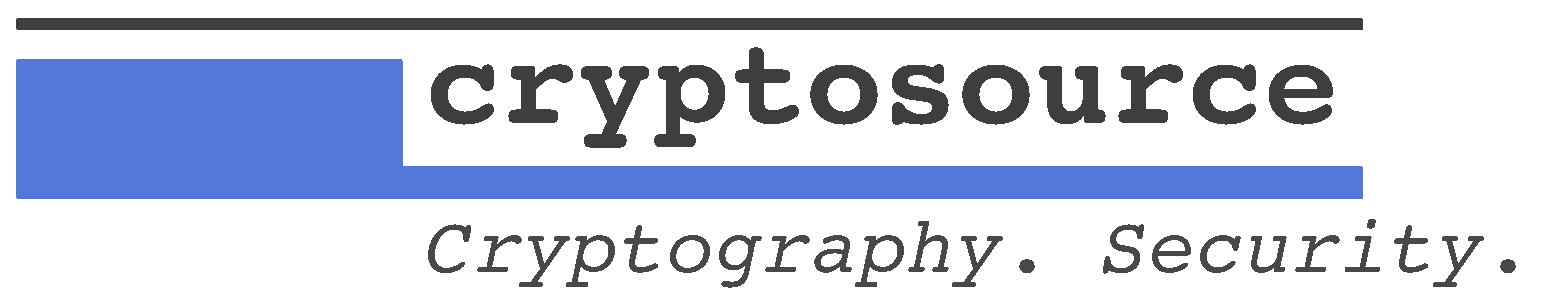
\includegraphics[width=6cm]{cs_logo.eps}}
\fancyhead[L]{flea cryptographic library 
\myVersion\\manual}
\fancyfoot[C]{\vspace{-0.3cm}\thepage}
\pagestyle{fancy}

%\ULWallPaper{bg.jpg}
\usepackage{eso-pic}
\newcommand\BackgroundIm{
  \put(5,-21){
    \parbox[b][\paperheight]{\paperwidth}{%
      \vfill
        \centering
        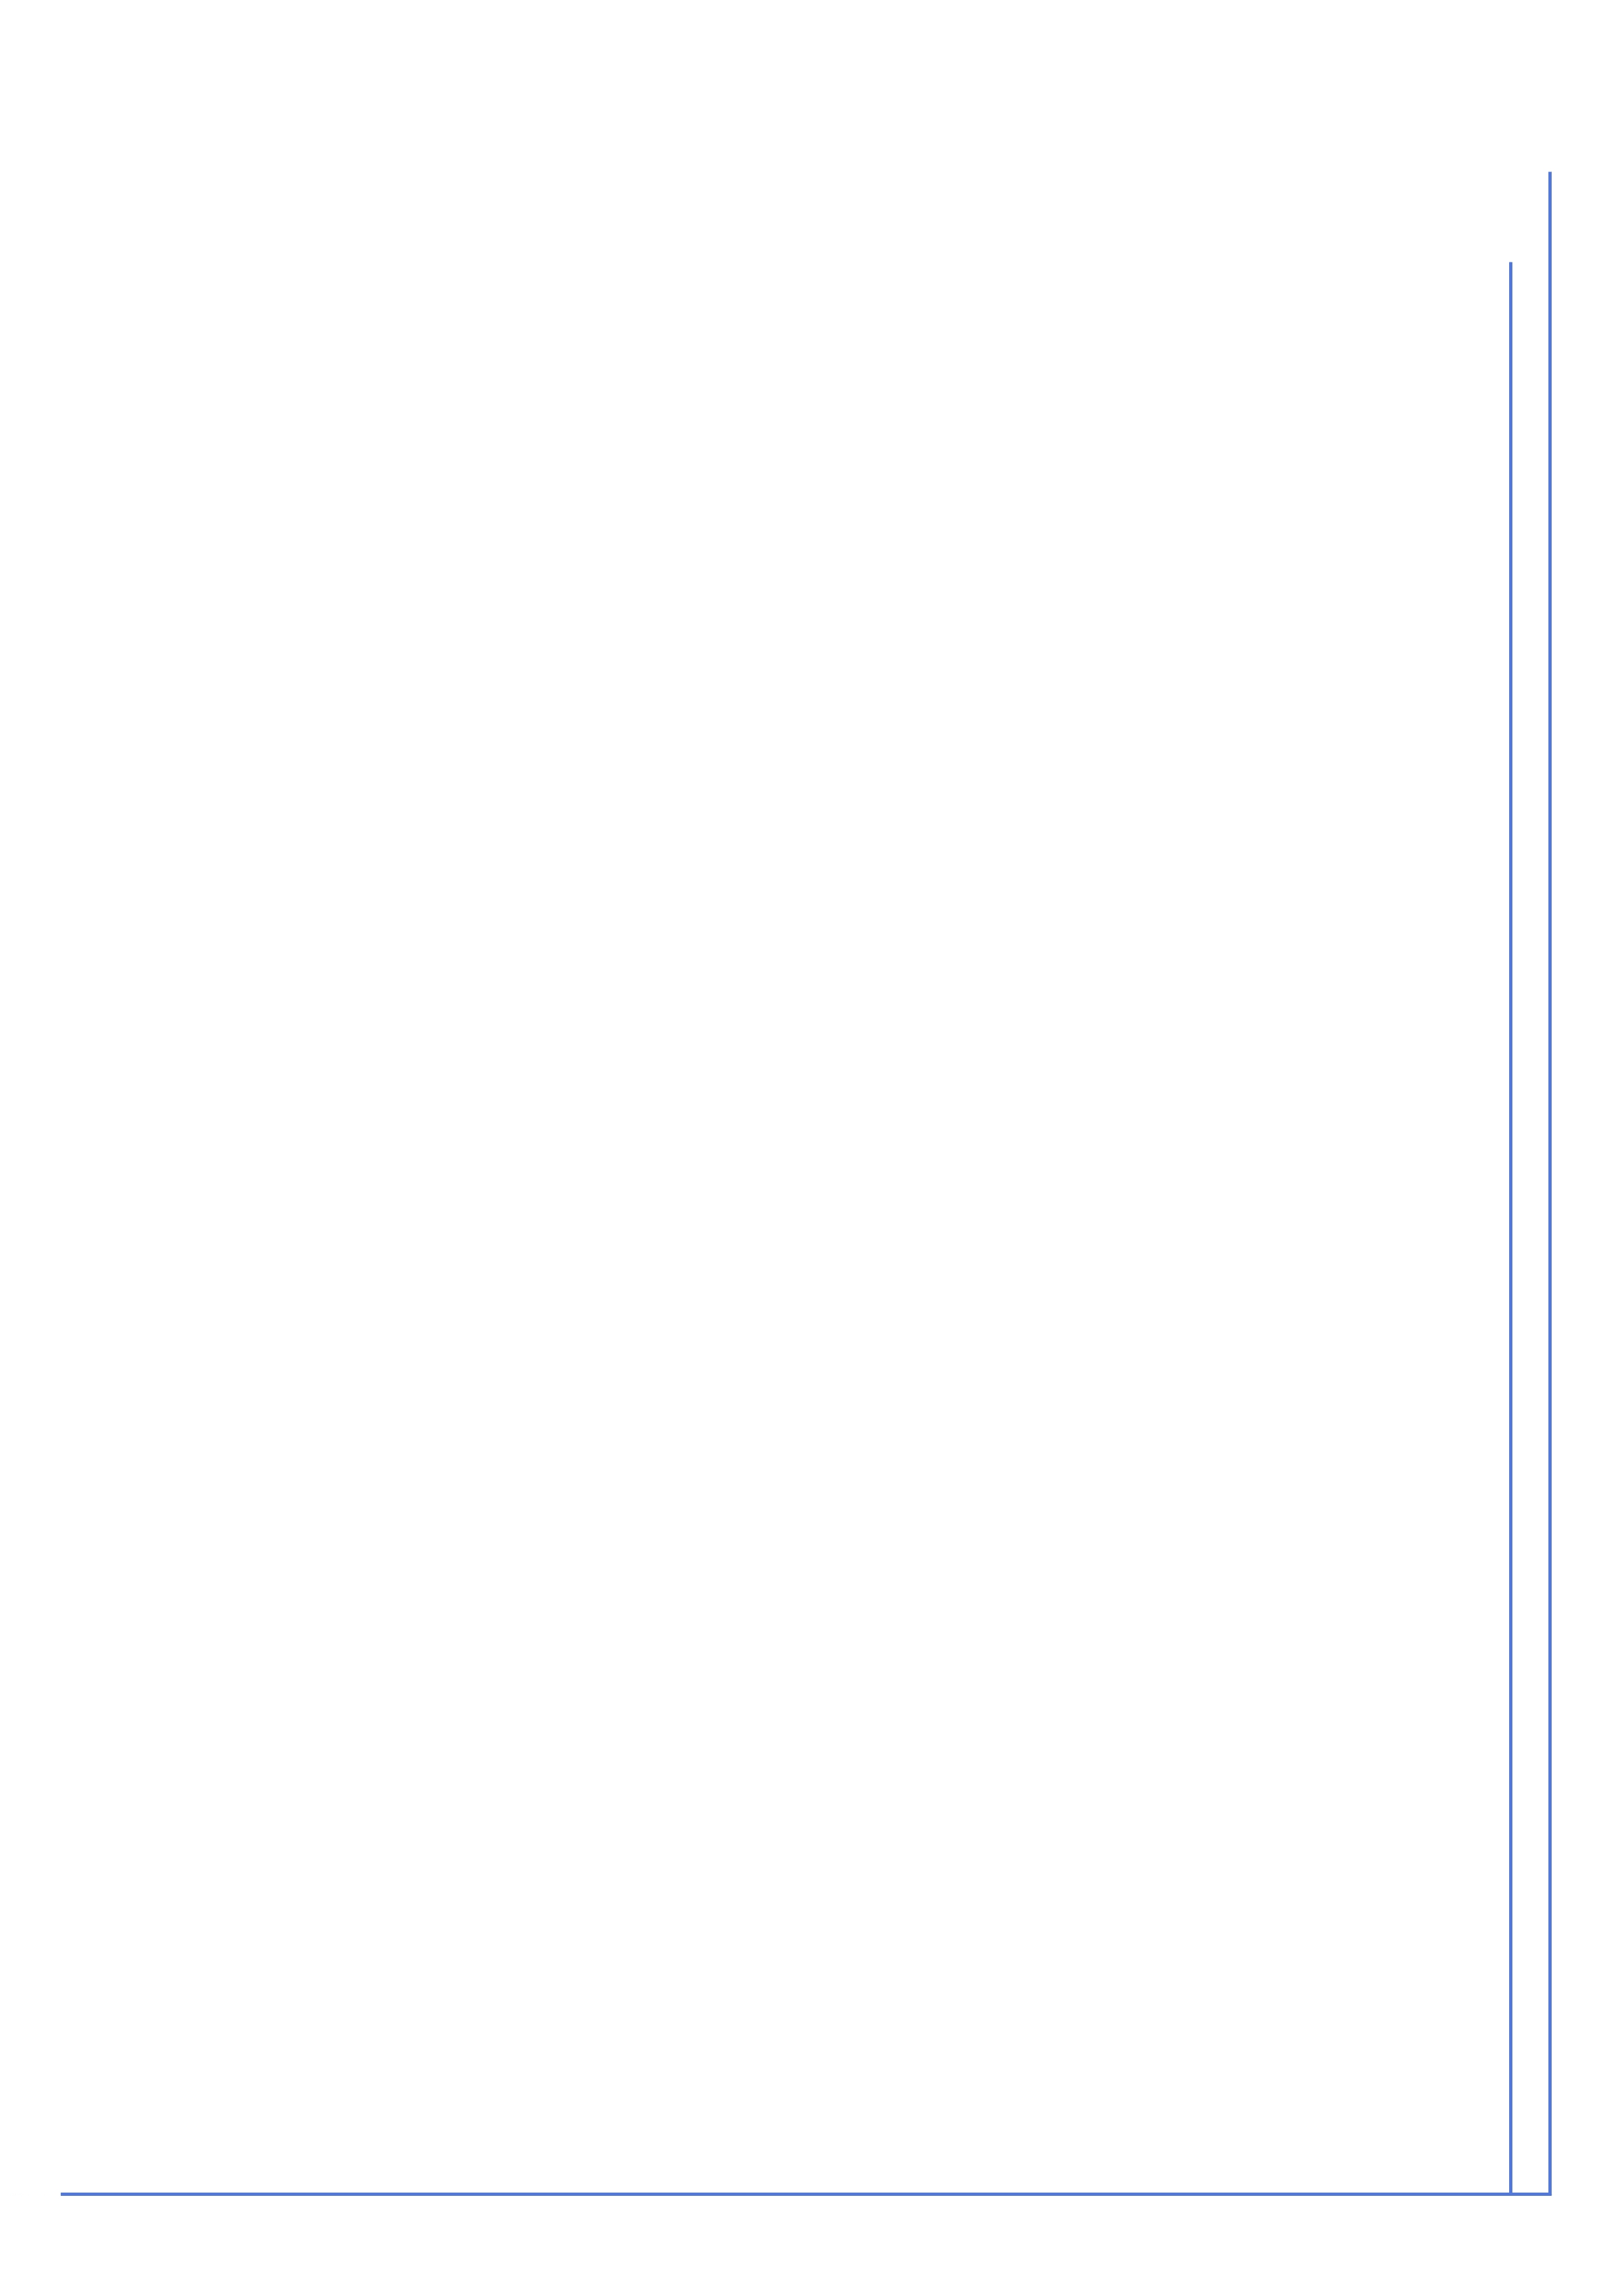
\includegraphics[height=\paperheight,width=\paperwidth,
        keepaspectratio]{bg.jpg}%
          \vfill
    }}}

        \renewcommand*\contentsname{\newline Contents}
\begin{document}
\AddToShipoutPicture{\BackgroundIm}
\changefont{cmss}{m}{n}
%\tikzset{XOR/.style={draw,circle,append after command={
%        [shorten >=\pgflinewidth, shorten <=\pgflinewidth,]
%        (\tikzlastnode.north) edge (\tikzlastnode.south)
%        (\tikzlastnode.east) edge (\tikzlastnode.west)
%        }
%    }
%}

\tikzstyle{manipblock} = [draw, fill=red!20, rectangle, 
    minimum height=2em, minimum width=6em]
\tikzstyle{origblock} = [draw, fill=green!20, rectangle, 
    minimum height=2em, minimum width=6em]
\tikzstyle{block} = [draw, fill=blue!20, rectangle, 
    minimum height=2em, minimum width=6em]
\tikzstyle{decbox} = [draw, fill=blue!20, rectangle, 
    minimum height=1em, minimum width=1em]
\tikzstyle{manipbytebox} = [draw, fill=red!20, rectangle, 
    minimum height=1em, minimum width=6em]
\tikzstyle{sum} = [draw, fill=blue!20, circle, node distance=1cm]

\newcommand{\myVersion}{v1.1 pre 2017-08-15}
%\mainmatter              % start of the contributions
%
\title{flea cryptographic library \myVersion\\{\LARGE manual} }

\author{cryptosource GmbH,
  Darmstadt\\\url{flea@cryptosource.de}\\\url{www.cryptosource.de}\vspace{0.5cm}\\
\includegraphics[width=7cm]{logo.png}}

\maketitle              % typeset the title of the contribution

%\begin{abstract}
%\end{abstract}

\newpage

\setcounter{tocdepth}{3}
\vspace{1cm}
\tableofcontents

\newpage

\section{Introduction}
flea, the acronym of ``flexible lightweight efficient algorithms'' is a
cryptographic library written in C and intended for resource
constrained devices. 
%In the current version it
%comes with a basic set of the most fundamental symmetric and asymmetric
%algorithms. 
It is especially intended to run on bare microcontrollers without
any operating system support. However, it can be readily run on standard PCs as
well. The current release of flea only supports 32-bit architectures but
compiles and runs also on 64-bit machines.


  \section{Getting started with flea}

  In order to get easily started with flea, the library is shipped with a CMake
  configuration to build it on standard Linux. In the
  flea directory, the command sequence 
  \begin{verbatim}
  cmake .
  make -j4
  ./build/unit_test
  \end{verbatim}
  can be issued to build the library, the unit tests, and execute the tests.

  However, the library is shipped in a state in which it produces two
  compilation errors. This is due to the fact that for the secure operation of
  the random number generator (RNG) of the library the user has to implement two
  functions for the persistence of the RNG state. The source code contains
  guidance how to quickly repair these compilation errors with a workaround,
  which, however, leads to an insecure build of the library that must not be
  used in production code. In Section \ref{secRng} we give guidance on how to use
  the RNG safely.

  \section{Compile-Time Configuration}

The library offers various compile-time
configuration options, such as 
\begin{itemize}
  \item the set of algorithms to include in the library
  \item use of stack memory only or the additional use of heap memory,
  \item configuration of the maximal key sizes for the determination of the
    buffer sizes in stack-only mode,
  \item buffer overwrite detection through canary values at the start and end of
    each buffer,
  \item various trade-offs concerning code-size, RAM demand and speed.
  \end{itemize}

  The compile-time configuration of the library is completely managed by a
  preprocessor framework. All configuration options can be set in the file
  \verb#build_cfg/general/build_config.h#, making it easy to configure the
  library on embedded platforms without any dependency on the build system.

  In order to build the library on an arbitrary 32-bit platform, the following
  directories must be in the compiler's include path:
  \begin{itemize}
    \item \verb#include#
    \item \verb#include/api#
    \item \verb#test/include# (in case that the unit tests shall be build)
    \item \verb#build_cfg/pltf_spec/32bit_default#
    \item \verb#build_cfg/general#
  \end{itemize}

\section{Random Number Generation }
\label{secRng}

flea features a simple but secure random number generator which is based on
the management of an RNG state file. In order to use the RNG safely in an
embedded firmware, the following steps must be taken. 

\subsection{Necessary Steps During Implementation}
During implementation, the in the file \verb#src/user/prng_user.c# the functions
for loading the PRNG state from the non-volatile memory (NVM)  and saving it to the NVM have to be
implemented. The developer must allocate an area within the device's NVM for
this purpose, the size of which is 32 bytes.

A second requirement is that during the device's startup, prior to the use of any
other functions of the flea library, the function 
\begin{verbatim}
flea_err_t THR_flea_lib__init()
\end{verbatim}
must be called, which internally loads the RNG state from NVM into the
corresponding RAM variable.


\subsection{Necessary Steps During Production and Activation}
When the devices running the firmware using flea are produced, before the
execution of any cryptographic operation, the PRNG state must be seeded with a
high entropy seed different for each device. 
%This seed should be generated on an
%external computer which has appropriate entropy sources available for this
%purpose. 
The function 
\begin{verbatim}
flea_err_t THR_flea_rng__reseed_persistent(const flea_u8_t* seed, flea_dtl_t seed_len);
\end{verbatim}
must be called once during the production or activation process with that seed data.
From that point on, the RNG state will be managed internally by the flea
library. During startup, when the function \verb#THR_flea_lib__init()# is
called, the stored RNG state is loaded from NVM to initialize the RNG, then a
fresh RNG state is created from the RNG's output and stored in the NVM. From
that point on, the RNG operates efficiently with its RAM state and secure,
non-repetitive random number generation is ensured even after a reset. 

\section{Using flea's API}

flea uses a macro framework to abstract object and buffer initialization as well
as error handling. This allows for greater flexibility and security for a number of reasons:
\begin{itemize}
  \item it is possible to switch between stack and heap usage for buffer allocation
  by changing a single compiler flag,
  \item the life cycles of buffers and objects are formalized and integrate
    seamless with the error handling, guaranteeing safety from resource leaks
    and errors such as use-after-free if the programming standards are adhered
    to.
\end{itemize}

From the following sections, only Sections \ref{secFleaObj} and \ref{secErrRet}
are essentially
important for users of the library since the other sections describe the
internal design of flea which is not necessary for the use of its API. But since
the test code shipped with flea, which can serve as a source of example code, is
written in the same framework, it is helpful to understand also the approaches
to error handling and buffer management outlined in the subsequent sections.
\subsection{flea's Objects}
\label{secFleaObj}
flea's objects have the following life cycle states:
\begin{itemize}
  \item \stateUninit. This state is entered by simply declaring an object on
    stack or heap without assigning any value to it. From this state, only the
    transition to the state \stateInit is allowed.
  \item \stateInit. This state is entered via one of the following means:
    \begin{itemize} 
        \item By using the macro
    \verb#FLEA_DECL_OBJ(symbol_name, object_type)# for the object declaration
    and simultaneous initialization. 
    \item Alternatively, an object in the state
    \stateUninit can make the transition to the state \stateInit by invoking the
    corresponding initialization macro.
    Their naming pattern is \verb#flea_<type>__INIT(symbol_address)#.
    In the state \stateInit, only two
    actions may be performed on the object: The object's destructor (dtor)
    function or one of its constructor (ctor) functions may be called.
\end{itemize}
  \item \stateCreated. This state can be entered in two ways
    \begin{itemize}
    \item By the calling one of the object's
    ctor functions or other functions which perform object creation. The state
    \stateCreated can only be left by calling the object's dtor function. If a
    function returns when any of its objects are in the state \stateCreated,
    then this will result in a memory leak in the case of heap mode.
    \item Alternatively, for some objects, the exist also initialization value
      macros labelled conforming to the naming pattern
      \verb#flea_<type>__CONSTR_<further specification>#. An object initialized
      with such a value is in the state \stateCreated afterwards.
  \end{itemize}
  \item \stateDestroyed. This state is entered by calling the object's dtor
    function. In this state, the dtor function may be called repeatedly (without
    any effect) or the object may be created again using a ctor function.
\end{itemize}

This is the contract offered by all class-like types of flea's API. The dtor calls should
be made even in the stack-only mode, because they wipe secret values from the
RAM before deallocation.

The flea library functions themselves realize an approach which ensures that all
requirements from flea life object cycle model are met. This approach is
described in Section \ref{fleaFuncSkel} and it is recommended to adapt it in implementations
using flea or realize a corresponding solution.


\subsection{Error Return Values}
\label{secErrRet}
Any function of flea that potentially returns an error, referred to as a throwing function, can be identified by starting with the string
\verb#THR_#. Such a function returns \verb#FLEA_ERR_FINE#, which is defined as
zero, upon success or one of the error codes define in \verb#flea/error.h# otherwise.
When calling throwing functions in flea it is necessary test their return value
and take appropriate actions if an error occured.

\subsection{Object Life Cycle and Error Handling within the flea Library Functions}
\label{fleaFuncSkel}
In order to establish a standardized and robust approach to object initialization,
object creation, object destruction and error handling, the flea library
function implementations themselves employ a dedicated macro framework. This
approach is described in the following to facilitate the understanding of the
implementation. Furthermore, it may be be adapted in the flea library user's own
code.

Specifically, any throwing function in flea is structured by the following skeleton:
\begin{verbatim}
  <declaration section>
  FLEA_THR_BEG_FUNC();
  <initialization section>
  <throwing section> 
  FLEA_THR_FIN_SEC(cleanup-code);
\end{verbatim}
In the \verb#declaration section# all variable declaration happen. Next, in the \verb#initialization section#  
all objects so far not initialized are initialized by means of the
corresponding initialization macros. Any throwing functions may only be called
after this section in the \verb#throwing section#. 
The \verb#cleanup-code# is the code that shall be executed whenever the function ends,
either by naturally running to the location of the macro call
\verb#FLEA_THR_FIN_SEC()# or because between the two macro calls an error was
thrown and not handled, causing an immediate jump to the cleanup-code. This can happen mainly due to two incidents:
\begin{itemize}
  \item An error was raised by calling the macro \verb#FLEA_THROW()#. This
    causes the routine to directly jump to the cleanup code and the function
    returns the error code raised by \verb#FLEA_THROW()#. 
  \item An error was returned by a throwing function called as
    \verb#FLEA_CCALL(THR_flea_some_function(args))#. The behaviour is the same
    as for the \verb#FLEA_THROW()# macro, i.e. a return value other than
    \verb#FLEA_ERR_FINE# causes an immediate jump to the cleanup-code. In this, the error code returned by the
    called function is returned by the current function.
\end{itemize}

It is important to stress that in order to have correct life cycle management even in the presence of errors
thrown directly in the code or returned by called functions, one essential rule must be followed:
Before any code is executed that potentially raises errors, all objects 
used within the function must have be initialized. 
  %  If only the \verb#FLEA_DECL_OBJ()# is used for the
  %  object declaration, then this is naturally achieved. 
    %If, however, any
    %objects are declared in the standard way and only initialized in the
    %initialization-section indicated above, then it is vital that no error
    %throwing code is executed in the initialization section.
%  \end{enumberate}
Following this rule ensures that the jump to the cleanup section, which
typically executes the dtors for all local objects, is possible at any time
during error-throwing code.

\subsection{Buffer Management}
The buffer management in flea is abstracted by macros in order to enable both
the abstraction from heap/stack usage and in order to enable the use of canary
values for buffer overwrite detection.

The following  macros are mainly employed for the buffer management:
\begin{itemize}
  \item \verb#FLEA_DECL_BUF(symbol_name, type, size)# declares a buffer, 
  \item \verb#FLEA_ALLOC_BUF(symbol_name, size)# allocates a buffer, 
  \item \verb#FLEA_FREE_BUF_FINAL(symbol_name)# frees a buffer,
  \item \verb#FLEA_FREE_BUF_SECRET_ARR(symbol_name, size)# also frees a buffer,
    but also overwrites the memory contents prior to that.
\end{itemize}
All buffer sizes are specified in element counts, not in bytes. However, the
user of the library, who does not intend to make use of flea's features for 
switching between stack and heap mode in his own code or use the buffer
canaries, may certainly use any explicit heap or stack buffer allocation as he
is used to.

\section{Support}
cryptosource provides commercial support for the flea library. Please visit
\url{http://cryptosource.de/product_flea_en.html} for further information or
contact us at \url{flea@cryptosource.de}.

\end{document}
